\documentclass[acmsmall]{ec19acm}

\settopmatter{printacmref=true}
\fancyhead{}
\copyrightyear{2019}
\acmYear{2019}
\setcopyright{rightsretained}
\acmConference[EC '19]{ACM EC '19: ACM Conference on Economics and Computation}{June 24--28, 2019}{Phoenix, AZ, USA}
\acmBooktitle{ACM EC '19: ACM Conference on Economics and Computation (EC '19), June 24--28, 2019, Phoenix, AZ, USA}
\acmDOI{10.1145/3328526.3329635}
\acmISBN{978-1-4503-6792-9/19/06}

\usepackage{tikz} % SW: Added for plots
\usepackage{subfiles}
\usepackage{wrapfig}
\usepackage[toc,page]{appendix}
\usepackage{url}            % simple URL typesetting
\usepackage{booktabs}       % professional-quality tables
\usepackage{nicefrac}       % compact symbols for 1/2, etc.
\usepackage{microtype}      % microtypography
\usepackage{amsmath,amssymb,amsfonts}
%\usepackage{natbib} % cannot use with AAAI! A.S.

\usepackage{amsthm} % The amsthm package provides extended theorem environments
\usepackage{float}
\usepackage{sgame, tikz} % Game theory packages
\usepackage{caption}
\usepackage{algorithm,algpseudocode}
\usepackage{makecell}
 \usepackage{multirow}
 \usepackage{graphicx}
\theoremstyle{definition}
%\newtheorem{definition}{Definition}
\newtheorem{finding}{Finding}
%\newtheorem{conjecture}{Conjecture}
\newtheorem{puzzle}{Puzzle}
\captionsetup{font=footnotesize}

% Alex' macro
\usepackage{xspace}
\newcommand{\OMIT}[1]{}
\newcommand{\xhdr}[1]{\vspace{1mm} \noindent{\bf #1}}
\newcommand{\ie}{{\em i.e.,~\xspace}}
\newcommand{\eg}{{\em e.g.,~\xspace}}

\newcommand{\term}[1]{\ensuremath{\mathtt{#1}}\xspace}
\newcommand{\TS}{\term{TS}}
\newcommand{\DEG}{\term{DEG}}
\newcommand{\DG}{\term{DG}}
\newcommand{\Beta}{\term{Beta}} % for Beta distribution
\newcommand{\Eeog}{\term{EoG}} % shorthand for "effective end of game"

\newcommand{\eps}{\varepsilon}

\newcommand{\MRV}{mean reward vector\xspace} % mean reward vector
\newcommand{\MRVs}{mean reward vectors\xspace} % mean reward vector

\newcommand{\HMR}{\term{HMR}}
\newcommand{\HM}{\term{HM}}
% a very useful package for edits and comments, from David Kempe (USC)
%\usepackage{color-edits}
\usepackage[suppress]{color-edits}  % use this to suppress the package
\addauthor{as}{red}    % as for Alex
\addauthor{ga}{blue}  % ga for Guy
\addauthor{sw}{orange} % sw for Steven
% e.g. for Alex, provides \asedit{}, \ascomment{} and \asdelete{}.
\setlength{\tabcolsep}{8pt} % Default value: 6pt
\renewcommand{\arraystretch}{1.5} % Default value: 1

%drt24 hacks
% Letter paper

% Hack to try to make acmart work with biblatex: https://tex.stackexchange.com/questions/37076/is-it-possible-to-load-biblatex-with-a-class-that-has-already-loaded-natbib
\let\citename\relax
%\RequirePackage[abbreviate=true, dateabbrev=true, isbn=true, doi=true, urldate=comp, url=true, maxbibnames=9, backref=false, backend=biber, style=ACM-Reference-Format, language=american]{biblatex}

\usepackage{booktabs} % For formal tables

\begin{document}
\title[The Perils of Exploration under Competition: A Computational Modeling Approach]
{The Perils of Exploration under Competition: \\ A Computational Modeling Approach}

\titlenote{Extended abstract. Full version is available as a technical report at \url{https://arxiv.org/abs/1902.05590}~.}

 \author{Guy Aridor}
 \affiliation{ \institution{Columbia University}}
 \author{Kevin Liu}
 \affiliation{\institution{Columbia University}}
 \author{Aleksandrs Slivkins}
 \affiliation{\institution{Microsoft Research, New York City}}
 \author{Zhiwei Steven Wu}
 \affiliation{\institution{University of Minnesota - Twin Cities}}



 \authorsaddresses{%
  Authors' addresses: Guy Aridor, Columbia University, New York, NY, g.aridor@columbia.edu; Kevin Liu, Columbia University, New York, NY, kevin.liu@columbia.edu; Aleksandrs Slivkins, Microsoft Research, New York, NY, slivkins@microsoft.com; Zhiwei Steven Wu, University of Minnesota - Twin Cities, Minneapolis, MN, zsw@umn.edu}

  \begin{CCSXML}
<ccs2012>
<concept>
<concept_id>10010405.10010455.10010460</concept_id>
<concept_desc>Applied computing~Economics</concept_desc>
<concept_significance>500</concept_significance>
</concept>
</ccs2012>
\end{CCSXML}

\ccsdesc[500]{Applied computing~Economics}

\fancyhead{}
%
% The code below should be generated by the tool at
% http://dl.acm.org/ccs.cfm
% Please copy and paste the code instead of the example below.
%
\keywords{Multi-armed bandits;Exploration;Competition;Competition vs Innovation}
\maketitle


We empirically study the interplay between \textit{exploration} and
  \textit{competition}. Systems that learn from interactions with
  users often engage in \emph{exploration}: making potentially
  suboptimal decisions in order to acquire new information for future
  decisions. However, when multiple systems are competing for
    the same market of users, exploration may hurt a system's
    reputation in the near term, with adverse competitive effects. In particular, a system may enter a ``death spiral", when the short-term reputation cost decreases
    the number of users for the system to learn from, which degrades the
    system's performance relative to competition and further decreases
    the market share.

We ask whether better exploration algorithms are incentivized under competition.  We run extensive numerical experiments in a stylized duopoly model, where two firms compete for users and simultaneously learn from them. Each firm commits to a multi-armed bandit algorithm, and \emph{explores} according to this algorithm. Users select between the two firms based on the current reputation score: rewards from the firm's algorithm, averaged over a recent time window. Each firm's objective is to maximize its market share (the fraction of users choosing this firm). We consider a \emph{permanent duopoly} in which both firms start at the same time, as well as \emph{temporary monopoly}: a duopoly with a first-mover. We focus on three classes of bandit algorithms, ranging from more primitive to more sophisticated: \emph{greedy algorithms} that do not explicitly explore, algorithms that separate exploration and exploitation, and algorithms that combine the two. We know from prior work that in the absence of competition,  ``better" algorithms are typcially better in the long run, but could be worse initially.


\tikzstyle{level 1}=[level distance=2.0cm, sibling distance=4.0cm]
\tikzstyle{level 2}=[level distance=2.0cm, sibling distance=2cm]
\tikzstyle{below} = [align=center]

\xhdr{Main findings.}
We find that in the permanent duopoly, competition incentivizes firms to choose the ``greedy algorithm", and even more so if the firm is a late arriver in a market. This algorithm also prevails under monopoly, simply because it tends to be easier to deploy. Whereas the incumbent in 
\begin{wrapfigure}{r}{0.5\textwidth}
\vspace{-2mm}
\begin{center}
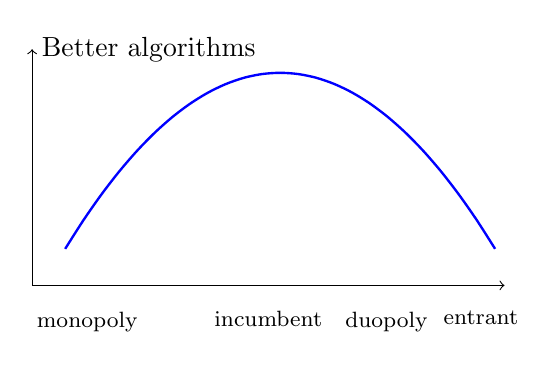
\begin{tikzpicture}
      \draw[->] (0,0) -- (6,0) node[right] {};
      \draw[->] (0,0) -- (0,3) node[right] {Better algorithms};
      \draw[scale=0.6,domain=0.7:9.8,smooth,variable=\x,blue, line width=0.3mm] plot ({\x},{4.5 - 0.18 * (\x - 5.25)^2});
     \node[below] at (0.7, -0.22) {\footnotesize monopoly};
     \node[below] at (3, -0.2) {\footnotesize incumbent};
     \node[below] at (4.5, -0.22) {\footnotesize duopoly};
     \node[below] at (5.7, -0.2) {\footnotesize entrant};
 \end{tikzpicture}
 \caption{A stylized ``inverted-U relationship" between strength of competition and ``level of innovation".}
\label{fig:inverted-U}
\end{center}
\end{wrapfigure}
the temporary monopoly is incentivized to deploy a more advanced exploration algorithm. As a result, consumer welfare is highest under temporary monopoly. We find strong evidence of the ``death spiral" effect mentioned earlier; it is strongest under permanent duopoly.


Interpreting the adoption of better algorithms as ``innovation", our findings can be framed in terms of the ``inverted-U relationship" between competition and innovation (see Figure~\ref{fig:inverted-U}). This is a well-established concept in the economics literature, dating back to \cite{Schumpeter-42}, whereby too little or too much competition is bad for innovation, but intermediate levels of competition tend to be better. However, the ``inverted-U relationship'' is driven by different aspects in our model than the ones in the existing literature in economics:  the barriers for innovations arise due to the reputational consequences of exploration rather than the R\&D costs.


\xhdr{Additional findings.}
We investigate the ``first-mover advantage" phenomenon in more detail. Being first in the market gives free data to learn from (a ``data advantage") as well as a more definite, and possibly better reputation compared to an entrant (a ``reputation advantage"). We run additional experiments so as to isolate and compare these two effects. We find that either effect alone leads to a significant advantage under competition. The data advantage is larger than reputation advantage when the incumbent commits to a more advanced bandit algorithm.

Data advantage is significant from the anti-trust perspective, as a possible barrier to entry. We find that even a small amount ``data advantage" gets amplified under competition, causing a large difference in eventual market shares. This observation runs contrary to prior work,  %\cite{varian2018artificial,lambrecht2015can,bajari2018impact},
which studied learning without competition, and found that small amounts of additional data do not provide significant improvement in eventual outcomes. We conclude that competition dynamics -- that firms compete as they learn over time -- are pertinent to these anti-trust considerations.

We also investigate how algorithms' performance ``in isolation" (without competition) is predictive of the outcomes under competition. We find that mean reputation -- arguably, the most natural performance measure ``in isolation" -- is sometimes not a good predictor. We suggest a
more refined performance measure, and use it to explain some of the competition outcomes.


We also consider an alternative choice rule with explicit noise/randomness: a small fraction of users choose a firm uniformly at random. We confirm the theoretical intuition that better algorithms prevail if the expected number of ``random" users is sufficiently large. However, we find that this effect is negligible for some smaller but still ``relevant" parameter values.


\xhdr{Discussion.}
Our paper is an experimental counterpart to \cite{CompetingBandits-itcs18}, which considered a similar duopoly model and obtained a number of theoretical results with ``asymptotic" flavor. For analytical tractability, \cite{CompetingBandits-itcs18} makes a somewhat unrealistic simplification that users do not observe any signals about firms' ongoing performance. The strength of competition is varied using assumptions about (ir)rational user behavior. For these reasons, the theorems from \cite{CompetingBandits-itcs18} have no direct bearing on our simulations. However, their high-level conclusion \gadelete{in} is an inverted-U relationship similar to ours.

The present paper provides a more nuanced and ``non-asymptotic" perspective. The reputation-based choice model accounts for competition in a more direct way, allows to separate reputation vs. data advantage, and makes our model amenable to numerical simulations (unlike the model in \cite{CompetingBandits-itcs18}).

\bibliographystyle{acm}
\bibliography{refs,bib-abbrv-short,bib-bandits,bib-AGT,bib-slivkins}


\end{document}
%%% Local Variables:
%%% mode: latex
%%% TeX-master: t
%%% End:
